% Copyright 2023-2024 Kieran W Harvie. All rights reserved.

\section{Simplicial Homology}
I need to revise Simplicial Homology so I'm going to give some definitions and then work some examples.

\subsection{Simplicial Definitions}

\subsubsection{Simplex:}
A simplex is a generalization of a triangle to higher/lower dimensions:

\begin{itemize}
	\item 0-simplex is a point
	\item 1-simplex is a segment
	\item 2-simplex is a triangle
	\item 3-simplex is a tetrahedron
\end{itemize}

For our purposes we specify a simplex with an ordered word written from the set of points.
For example $a$ is a point, $bc$ is a segment, and $abc$ is a triangle:
\begin{center}
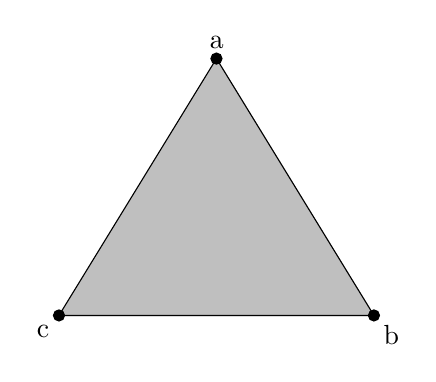
\begin{tikzpicture}
	\filldraw[lightgray] (-2,0)  --(2,0)--(0,3.26210161512);
	\draw (-2,0)--(2,0)--(0,3.26210161512)--(-2,0);
	\filldraw (-2,0) node[below left] {c} circle (2pt);
	\filldraw (2,0) node[below right] {b} circle (2pt);
	\filldraw (0,3.26210161512) node[above] {a} circle (2pt);
\end{tikzpicture}
\end{center}
Two important remarks.
Firstly, $abc\neq acb$ the former one goes around counter-clockwise and the later clockwise.
Secondly, the set $\{ab,bc,bc\}$ is not a triangle and is not the same as $abc$ or $\{abc\}$.
It's all the edges of a triangle but not its interior.

\subsubsection{Face:}
$n$ 0-simplexes defines a $n$-simplex and is called the face of the points.
Conversely the vertices that define a simplex and all the faces that come from that simplex are called the faces of the original simplex.

\subsubsection{Geometric Simplicial Complex}
A Geometric Simplicial Complex $\mathcal{K}$ is a set of simplexes such that:
\begin{enumerate}
	\item Every face of an element of $\mathcal{K}$ is also an element of $\mathcal{K}$.
	\item The non-empty intersection of two simplexes $\sigma_0,\,\sigma_1\in\mathcal{K}$ is a face of both $\sigma_1$ and $\sigma_0$.
\end{enumerate}

\subsubsection{Chain}
A $k$-chain of $\mathcal{K}$ is a formal linear sum of $k$-simplexes.
A $2$-chain is naturally interpreted as a,
possible disconnected and repeated, 
path through $\mathcal{K}$.
\\

More formally, 
given a complex $\mathcal{K}$ the group of $n$-chain $C_n(\mathcal{K})$ is a free $\mathbb{Z}$-module over the $n$-simplexes where two simplexes are equal if they have the same orientation\footnote{The words are even permutation of each other.} and additive inverse if opposite.
(Define $C_{-1} = 0$ for convenience).
\\

For example: $ab+bc$ is the path from $a$ to $c$ through $b$,
$abc = -acb$ are the same triangle with different handedness,
$2ab+dc$ is going over $ab$ twice then jumping to $dc$.
\\

Although the lower dimensions have intuitive geometric interpretation the whole configuration can more intuitively viewed as a combinatoric exercise. 

\subsection{Homology Definitions}
\subsubsection{Boundary Operator}
Given a simplex $\sigma$ define $\sigma_k$ as the same word a $\sigma$ with the $k^\text{th}$ point removed.
The boundary operator $\partial_k:C_k\rightarrow C_{k-1}$ is defined as:
\[\partial_k(\sigma) = \sum_{i=0}^k(-1)^i\sigma_i\]
The boundary of a $0$-simplex is $0$,
the boundary of a $1$-simplex is final point minus inital,
the boundary of a $2$-simplex is it's normal boundary (hence the name).
\\

\begin{equation*}
\begin{aligned}
	\partial_0(a) &= 0\\
	\partial_1(ab) &= b-a\\
	\partial_2(abc) &= ac + cb + bc\\
\end{aligned}
\end{equation*}

\subsubsection{Cycles Subgroup}
The cycles subgroup, $Z_n$, of $C_n$ is the kernel of $\partial_n$:
\[ Z_n = \ker\partial_n\]

The name comes from the $n=1$ case where a $x\in\ker\partial_n$ iff the $1$-chain is cyclic path.

\subsubsection{Boundaries Subgroup}
The boundaries subgroup, $B_n$, of $C_n$ is the image of $\partial_{n+1}$:
\[ B_n = \img\partial_{n+1}\]

The name comes from the $n=1$ case where $\partial_2(x)$ is a $1$-chain going over the boundary of $x$.

\subsubsection{Homology Group}
The boundary of a boundary is $0$.
For intuition consider the $n=1$ case,
the boundary is a cyclic path and hence the boundary of a boundary is zero.
\\

In the general case the boundary of the boundary of $\sigma$ is a sum of words of $\sigma$ with two letters removed where each word appears twice,
once for when the earlier letter is removed first then the last and again in the opposite order.
Let $\sigma_{i,j}$ be the word obtained removing the $i^\text{th}$ and $j^\text{th}$ letter.

When $i< j$ we have:
\[\sigma_{i,j} = (\sigma_i)_j\]
Since taking $i^\text{th}$ out first doesn't effect removing $j^\text{th}$.
And when taking the $j^\text{th}$ element first means the $i^\text{th}$ element is now one letter over:
\[\sigma_{i,j} = (\sigma_j)_{i-1}\]

Now observe that for the sum for the boundary of th boundary:
\begin{equation*}
\begin{aligned}
	\partial_k(\partial_{k+1}(\sigma)) =& \sum_{i=0}^{k}(-1)^i\sum_{j=0}^{k+1}(-1)^j(\sigma_j)_i\\
	=& \sum_{i=0}^{k}\sum_{j=0}^{k+1}(-1)^{i+j}(\sigma_j)_i\\
\end{aligned}
\end{equation*}
Meaning the $j-1$ in the index of the $j$ first case changes the sign of $\sigma_{i,j}$ compared to the $i$ first case.
Hence the terms cancel and the sum is zero.
\\

A direct consequence is that $\img\partial_{n+1}$ is a normal subgroup of $\ker\partial_n$ meaning we can use the fundamental isomorphism theorem to define the quotient group:
\[H_n(\mathcal{K}) = \frac{Z_n}{B_n} = \frac{\ker\partial_n}{\img\partial_{n+1}}\]

\subsection{Worked Examples}
\subsubsection{Disconnected example}
\begin{center}
\begin{tikzpicture}
	\draw (2,0)--(0,3.26210161512);
	\filldraw (-2,0) node[below left] {c} circle (2pt);
	\filldraw (2,0) node[below right] {b} circle (2pt);
	\filldraw (0,3.26210161512) node[above] {a} circle (2pt);
\end{tikzpicture}
\end{center}
\[\mathcal{K}=\{a,b,c,ab\}\]
There's no simplexes of dimensions larger than $3$ hence $C_{n\geq 3} = 0$ and $H_{n\geq 2}(\mathcal{K}) = 0$.
Hence we have:
\[0 \stackrel{\partial_2}{\longrightarrow} C_1 \stackrel{\partial_1}{\longrightarrow} C_0 \stackrel{\partial_0}{\longrightarrow} 0\]
Where:
\[C_1 = \langle ab \rangle,\quad C_0 = \langle a,b,c \rangle\]
All results are pretty trivial:
\begin{equation*}
\begin{aligned}
	&\img \partial_2 = 0 && \ker \partial_1 = 0\\
	&\img \partial_1 = \langle a-b\rangle && \ker \partial_0 = \langle a,b,c\rangle\\
\end{aligned}
\end{equation*}
Gives the homologies:
\begin{equation*}
\begin{aligned}
	H_0(\mathcal{K}) =& \frac{\ker\partial_0}{\img\partial_1} = \frac{\langle a,b,c\rangle}{\langle a-b\rangle} = \langle a,c\rangle = \mathbb{Z}^2\\
	H_1(\mathcal{K}) =& \frac{\ker\partial_1}{\img\partial_2} = 0 \\
\end{aligned}
\end{equation*}


\subsubsection{Triangle without Interior}
\begin{center}
\begin{tikzpicture}
	\draw (-2,0)--(2,0)--(0,3.26210161512)--(-2,0);
	\filldraw (-2,0) node[below left] {c} circle (2pt);
	\filldraw (2,0) node[below right] {b} circle (2pt);
	\filldraw (0,3.26210161512) node[above] {a} circle (2pt);
\end{tikzpicture}
\end{center}
\[\mathcal{K}=\{a,b,c,ab,ac,bc\}\]

Like with the previous example $H_{n\geq 2}(\mathcal{K}) = 0$.
Hence we have:
\[0 \stackrel{\partial_2}{\longrightarrow} C_1 \stackrel{\partial_1}{\longrightarrow} C_0 \stackrel{\partial_0}{\longrightarrow} 0\]
Where:
\[C_1 = \langle ab,ac,bc \rangle,\quad C_0 = \langle a,b,c \rangle\]
The $\ker$ and $\img$ are given bellow:
\begin{equation*}
\begin{aligned}
	&\img \partial_2 = 0 && \ker \partial_1 = \langle ab+bc+ca\rangle\\
	&\img \partial_1 = \langle a-b,a-c,b-c\rangle && \ker \partial_0 = \langle a,b,c\rangle\\
\end{aligned}
\end{equation*}

Proof for $\ker \partial_1$
\begin{equation*}
\begin{aligned}
	&\partial_1(\alpha\,ab+\beta\,bc+\gamma\,ca)\\
	=&\alpha(a-b)+\beta(b-c)+\gamma(c-a) \\
	=&(\alpha-\gamma)a+(-\alpha+\beta)b+(-\beta + \gamma)c \\
\end{aligned}
\end{equation*}
It might already be intuative that you can only choose one of $\alpha,\beta,\gamma$ then the rest are fixed.
But you can also use the following module equation:
\[
	\begin{bmatrix}
		1&0&-1\\
		-1&1&0\\
		0&-1&1\\
	\end{bmatrix}
	\begin{bmatrix}
		\alpha\\
		\beta\\
		\gamma\\
	\end{bmatrix}
	=
	\begin{bmatrix}
		0\\0\\0\\
	\end{bmatrix}
\]

Gives the homologies:
\begin{equation*}
\begin{aligned}
	H_0(\mathcal{K}) =& \frac{\ker\partial_0}{\img\partial_1} = \frac{\langle a,b,c\rangle}{\langle a-b,a-c,b-c\rangle} = \langle a\rangle = \mathbb{Z}\\
	H_1(\mathcal{K}) =& \frac{\ker\partial_1}{\img\partial_2} = \frac{\langle ab+bc+ca\rangle}{0} =\langle ab+bc+ca\rangle =\mathbb{Z}\\
\end{aligned}
\end{equation*}

\subsubsection{Triangle with Interior}
\begin{center}
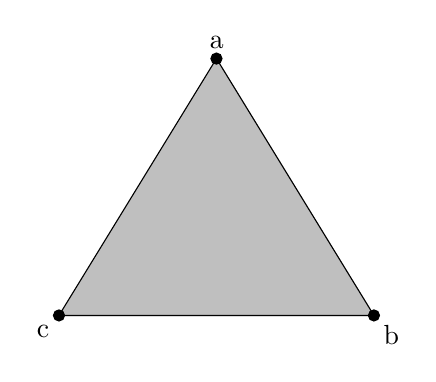
\begin{tikzpicture}
	\filldraw[lightgray] (-2,0)--(2,0)--(0,3.26210161512);
	\draw (-2,0)--(2,0)--(0,3.26210161512)--(-2,0);
	\filldraw (-2,0) node[below left] {c} circle (2pt);
	\filldraw (2,0) node[below right] {b} circle (2pt);
	\filldraw (0,3.26210161512) node[above] {a} circle (2pt);
\end{tikzpicture}
\end{center}
\[\mathcal{K}=\{a,b,c,ab,ac,bc,abc\}\]

There are no simplexes with order larger than $3$ hence like in previous examples $H_{n\geq 3}(\mathcal{K}) = 0$.
Hence we have:
\[0 \stackrel{\partial_3}{\longrightarrow} C_2 \stackrel{\partial_2}{\longrightarrow} C_1 \stackrel{\partial_1}{\longrightarrow} C_0 \stackrel{\partial_0}{\longrightarrow} 0\]
Where:
\[C_2 = \langle abc \rangle,\quad C_1 = \langle ab,ac,bc \rangle,\quad C_0 = \langle a,b,c \rangle\]
The $\ker$ and $\img$ are given bellow:
\begin{equation*}
\begin{aligned}
	&\img \partial_3 = 0 && \ker \partial_2 = 0\\
	&\img \partial_2 = \langle ab+bc+ca\rangle && \ker \partial_1 = \langle ab+bc+ca\rangle\\
	&\img \partial_1 = \langle a-b,a-c,b-c\rangle && \ker \partial_0 = \langle a,b,c\rangle\\
\end{aligned}
\end{equation*}

Gives the homologies:
\begin{equation*}
\begin{aligned}
	H_0(\mathcal{K}) =& \frac{\ker\partial_0}{\img\partial_1} = \frac{\langle a,b,c\rangle}{\langle a-b,a-c,b-c\rangle} = \langle a\rangle = \mathbb{Z}\\
	H_1(\mathcal{K}) =& \frac{\ker\partial_1}{\img\partial_2} = \frac{\langle ab+bc+ca\rangle}{\langle ab+bc+ca\rangle} = 0\\
	H_2(\mathcal{K}) =& \frac{\ker\partial_2}{\img\partial_3} = \frac{0}{0} = 0\\
\end{aligned}
\end{equation*}

\subsection{More Worked Examples}
\subsubsection{Tetrahedron without interior:}
\begin{center}
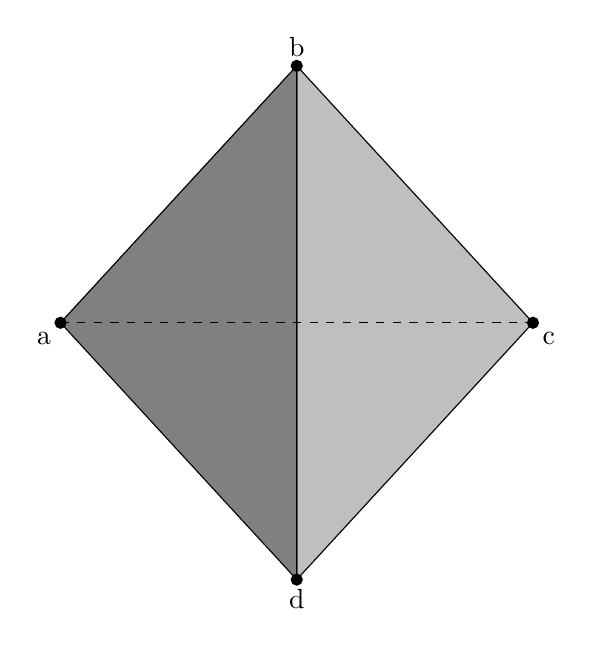
\begin{tikzpicture}
	\filldraw[gray] (-3,0)--(0,3.26210161512)--(0,-3.26210161512);
	\filldraw[lightgray] (0,3.26210161512)--(3,0)--(0,-3.26210161512);
	\draw (-3,0)--(0,3.26210161512)--(0,-3.26210161512)--(-3,0);
	\draw (3,0)--(0,3.26210161512)--(0,-3.26210161512)--(3,0);
	\draw[dashed] (-3,0)--(3,0);
	\filldraw (-3,0) node[below left] {a} circle (2pt);
	\filldraw (0,3.26210161512) node[above] {b} circle (2pt);
	\filldraw (0,-3.26210161512) node[below] {d} circle (2pt);
	\filldraw (3,0) node[below right] {c} circle (2pt);
\end{tikzpicture}
\end{center}
\[\mathcal{K}=\{a,b,c,d,ab,ac,ad,bc,cd,db,abc,abd,acd,cdb\}\]

We have:
\[0 \stackrel{\partial_3}{\longrightarrow} C_2 \stackrel{\partial_2}{\longrightarrow} C_1 \stackrel{\partial_1}{\longrightarrow} C_0 \stackrel{\partial_0}{\longrightarrow} 0\]
Where:
\[C_2 = \langle abc,abd,acd,cbd \rangle,\quad C_1 = \langle ab,ac,ad,bc,bd,dc, \rangle,\quad C_0 = \langle a,b,c \rangle\]
The $\ker$ and $\img$ are larger than previous examples,
despite being simplified,
and are given bellow:
\begin{equation*}
\begin{aligned}
	\img \partial_3 &= 0 \\
	\img \partial_2 &= \langle ab+bc+ca,ab+bd+da,ac+cd+da\rangle\\ 
	\img \partial_1 &= \langle a-b,a-c,a-d\rangle\\
	\ker \partial_2 &= \langle abc+adb+adc+dcb\rangle\\
	\ker \partial_1 &= \langle ab+bc+ca,ab+bd+da,ac+cd+da\rangle\\
	\ker \partial_0 &= \langle a,b,c,d\rangle\\
\end{aligned}
\end{equation*}

Gives the homologies:
\begin{equation*}
\begin{aligned}
	H_0(\mathcal{K}) =& \frac{\ker\partial_0}{\img\partial_1} = \frac{\langle a,b,c,d\rangle}{\langle a-b,a-c,a-d\rangle} = \mathbb{Z}\\
	H_1(\mathcal{K}) =& \frac{\ker\partial_1}{\img\partial_2} = \frac{\langle ab+bc+ca,ab+bd+da,ac+cd+da\rangle}{\langle ab+bc+ca,ab+bd+da,ac+cd+da\rangle} = 0\\
	H_2(\mathcal{K}) =& \frac{\ker\partial_2}{\img\partial_3} = \frac{\langle abc+adb+adc+dcb\rangle}{0} = \mathbb{Z}\\
\end{aligned}
\end{equation*}

\subsubsection{Mixed}
\begin{center}
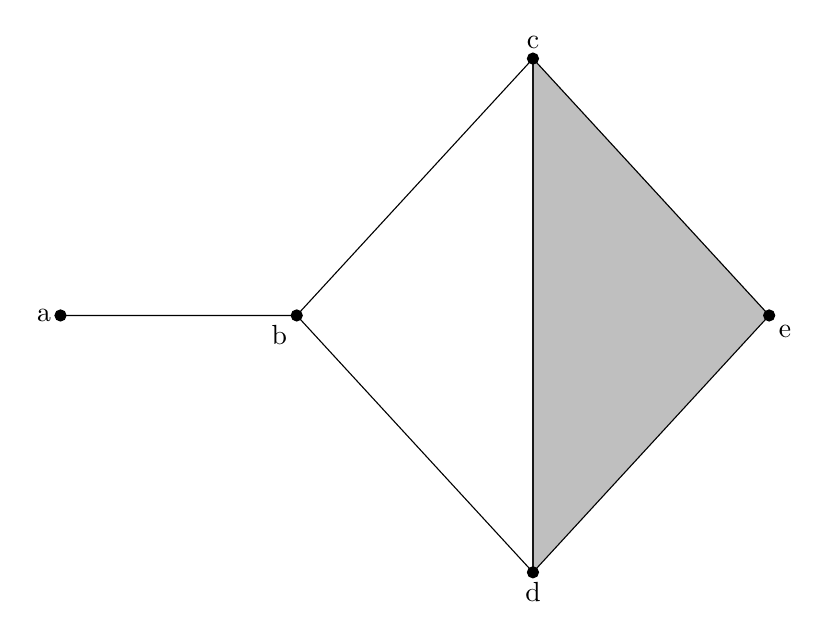
\begin{tikzpicture}
	\filldraw[lightgray] (3,0)--(0,3.26210161512)--(0,-3.26210161512);
	\draw (-6,0)--(-3,0)--(0,3.26210161512)--(0,-3.26210161512)--(-3,0);
	\draw (3,0)--(0,3.26210161512)--(0,-3.26210161512)--(3,0);
	\filldraw (-6,0) node[left] {a} circle (2pt);
	\filldraw (-3,0) node[below left] {b} circle (2pt);
	\filldraw (0,3.26210161512) node[above] {c} circle (2pt);
	\filldraw (0,-3.26210161512) node[below] {d} circle (2pt);
	\filldraw (3,0) node[below right] {e} circle (2pt);
\end{tikzpicture}
\end{center}
\[\mathcal{K}=\{a,b,c,d,e,ab,bc,bd,cd,ec,de,cde\}\]

We have:
\[0 \stackrel{\partial_3}{\longrightarrow} C_2 \stackrel{\partial_2}{\longrightarrow} C_1 \stackrel{\partial_1}{\longrightarrow} C_0 \stackrel{\partial_0}{\longrightarrow} 0\]
Where:
\[C_2 = \langle cde \rangle,\quad C_1 = \langle ab,bc,bd,cd,ec,de \rangle,\quad C_0 = \langle a,b,c,d,e \rangle\]
The $\ker$ and $\img$ are given bellow:
\begin{equation*}
\begin{aligned}
	&\img \partial_3 = 0 && \ker \partial_2 = 0\\
	&\img \partial_2 = \langle ce+ed+dc\rangle && \ker \partial_1 = \langle bc+cd+db, ce+ed+dc\rangle\\
	&\img \partial_1 = \langle a-b,b-c,b-d,c-d,e-c,d-e \rangle && \ker \partial_0 = \langle a,b,c,d,e\rangle\\
\end{aligned}
\end{equation*}

Gives the homologies:
\begin{equation*}
\begin{aligned}
	H_0(\mathcal{K}) =& \frac{\ker\partial_0}{\img\partial_1} = \frac{\langle a,b,c,d,e\rangle}{\langle a-b,b-c,b-d,c-d,e-c,d-e\rangle} = \langle a\rangle = \mathbb{Z}\\
	H_1(\mathcal{K}) =& \frac{\ker\partial_1}{\img\partial_2} = \frac{\langle bc+cd+db,ce+ed+dc\rangle}{\langle ce+ed+dc\rangle} = \langle bc+cd+db\rangle = \mathbb{Z}\\
	H_2(\mathcal{K}) =& \frac{\ker\partial_2}{\img\partial_3} = \frac{0}{0} = 0\\
\end{aligned}
\end{equation*}

\subsection{Interpretation of Simplicial Homology}
Let us summarise the worked example results:
\begin{center}
\begin{tabular}{|c|cccc|}
	\hline
	Complex & $H_0$ & $H_1$ & $H_2$ & $H_{n\geq 3}$ \\ 
	\hline
	Disconnected& $\mathbb{Z}^2$ &0&0&0 \\
	Triangle without interior& $\mathbb{Z}$ & $\mathbb{Z}$ & 0 & 0 \\
	Triangle with interior& $\mathbb{Z}$ & $0$ & 0 & 0 \\
	\hline
	\hline
	Tetrahedron without interior&$\mathbb{Z}$&0&$\mathbb{Z}$&0\\
	Mixed&$\mathbb{Z}$&$\mathbb{Z}$&0&0\\
	\hline
\end{tabular}
\end{center}
But what do they mean?
In a nutshell the power of $\mathbb{Z}$ corresponds to a specific topological feature called an $n$-hole.
A $0$-hole is a connected part,
a $1$-hole is a regular hole,
a $2$-hole is a cavity.
Hence the disconnected complex is made from two connected parts and the rest of one connected part.
And the triangle without an interior has a hole and the others don't.
\\

But why powers of  $\mathbb{Z}$?
And why does $\ker\partial_n / \img\partial_{n+1}$ give this result?
\\

The rigorous answer has to do with homotopy,
and the "Fundamental Homotopy Group" in particular,
which is the math of drawing loops on things then pulling them and then seeing where they get stuck.
Well worth a read but the basics are this:

For every hole you can wrap a loop around it multiple times and in both directions.
Wrapping it around clockwise once is identified with $1$,
wrapping it around counter-clockwise twice is identified with $-2$,
wrapping it around no hole is identified with $0$ since when the loop is pulled taut nothing gets stuck.

If there are two hole $a$ and $b$ then the loops are identified with an element over the free $\mathbb{Z}$-module over $\{a,b\}$.
For example $a+2b$ a clockwise loop over $a$ then two over $b$ and you can add two elements by making a cut in both loops then gluing them together (making sure you preserve orientation).

\begin{center}
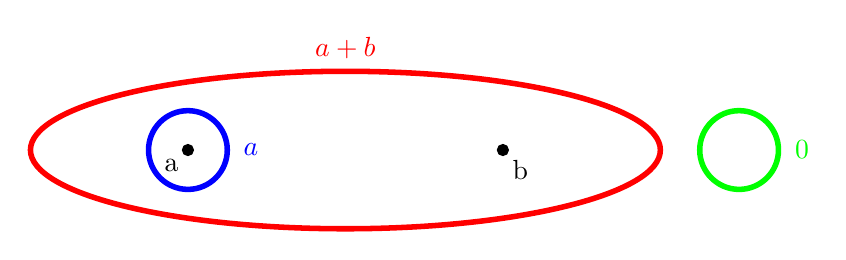
\begin{tikzpicture}
	\filldraw (-2,0) node[below left] {a} circle (2pt);
	\filldraw (2,0) node[below right] {b} circle (2pt);
	\draw[blue,line width=2pt] (-2,0) circle  [radius = 0.5cm];
	\draw[green,line width=2pt] (5,0) circle  [radius = 0.5cm];
	\draw[red,line width=2pt] (0,0) circle [x radius =4cm, y radius = 1cm];
	\node[blue] at (-1.2,0) {$a$};
	\node[green] at (5.8,0) {$0$};
	\node[red] at (0,1.3) {$a+b$};
\end{tikzpicture}
\end{center}

The free $\mathbb{Z}$-module over $\{a,b\}$ is isomorphic to $\mathbb{Z}^2$ because you need two integers to explain all the loops you can make over two holes that stay when taut,
which explains where the powers of $\mathbb{Z}$ came from.

$\ker\partial_n / \img\partial_{n+1}$ works because as noted in the definition of the chain group the elements of the chain group can jump around a bit.
But the requirement $\sigma\in\ker\partial_n$ makes it loop since it's boundary vanishes.
And $\img\partial_{n+1}$ are all the loops that have a higher order faces enabling a taut loop to move freely.
These steps combined give:
\begin{enumerate}
	\item $C_n$ contains all the loops but also completely broken path.
	\item Use $\ker\partial_n$ to get all elements of $C_n$ that are loops.
	\item Modulo $\img\partial_{n+1}$ to remove all loops that don't exit when pulled taut.
\end{enumerate}
\mbox 
Again, this explanation can be made more rigorous by studying homotopy.

\subsection{Boundaries and Cycles}
This is actually obvious,
but applying fundamental isomorphism theorem to $\partial_n:C_n\rightarrow C_{n-1}$ gives:
\[ B_{n-1} = \img\partial_n\cong \frac{C_n}{\ker\partial_n} = \frac{C_n}{Z_n} \]
This gives a new way to interpret $B_n$ based on $Z_n$,
and for $Z_n$ we only need to interpret $\sum_i (-1)^i\sigma_i =0$.
\\

It also makes me aware of how messy boundaries can be\footnote{And in math as well!}.
For example $\{ab,bc\}\subseteq C_1$ means $2a-b-c$ is and element of $B_0$ since you can take a chain of the edge from $b$ to $a$ and $c$ to $a$.
